\section*{B – Function fitting}

\subsection*{B.1 – Fitting a GP with Pyro}
\begin{itemize}
    \item Skal vi alternativt have én chain med 500 samples for final MCMC samples, og så bare bruge 4 chains til MCMC diagnostics? Lige nu bruger vi også 4 MCMC chains for final sample.
\end{itemize}
We are considering a hierarchical model in which we want to compute the predictive posterior distribution, $p(f^*|x^*,\mathcal{D})$. By \autoref{appendix1} we can approximate the posterior predictive by computing MCMC samples from the posterior, $p(\bm{\theta}|\mathcal{D})$, and thereafter averaging over $p(f^*|x^*,\mathcal{D},\bm{\theta}^{(i)})$:
\begin{equation}
    p(f^*|x^*,\mathcal{D})\approx N^{-1}\sum_{i=1}^Np(f^*|x^*,\mathcal{D},\bm{\theta}^{(i)})
\end{equation}
In order to reflect the true underlying posterior predictive, we should choose a sufficient amount of MCMC samples. To obtain MCMC samples from the target distribution, $p(\bm{\theta}|\mathcal{D})$, we require a sufficient warm-up period to ensure that the Markov chain has converged to its stationary distribution, which by construction is the target distribution. Further, the samples collected after the warm-up period should ideally have low autocorrelation in order to mimic the i.i.d. property as much as possible for a good distributional approximation. For this to occur, the chain should "mix well". We can assess convergence and mixing properties of the Markov chain generated by NUTS via inspection of trace plots, $\hat{R}$, and ESS. Using four chains we generate $4\cdot125=500$ samples without warm-up, where initial states of the Markov chains are chosen by random according to $p(\bm{\theta})$. The diagnostics are shown in \autoref{appendix2}. If we inspect the trace plot in \autoref{fig:mcmcdiag}, it appears that the typical set of $p(\bm{\theta}|\mathcal{D})$ is close to the typical set of $p(\bm{\theta})$, since the chains converge to the same stationary distribution within a few iterations. Thus, a warm-up period of 10 samples should be more than sufficient. Further, the trace plots indicate that the samples appear to be somewhat autocorrelated, which is supported by the values of $\hat{R}$ and ESS in \autoref{tab:mcmcdiag}. If one is concerned that this may result in a poor approximation, a remedy is to simply collect more samples. Since the number of samples is fixed to 500, we take the view that 500 samples offers a good approximation.

\begin{figure}[H]
    \centering
    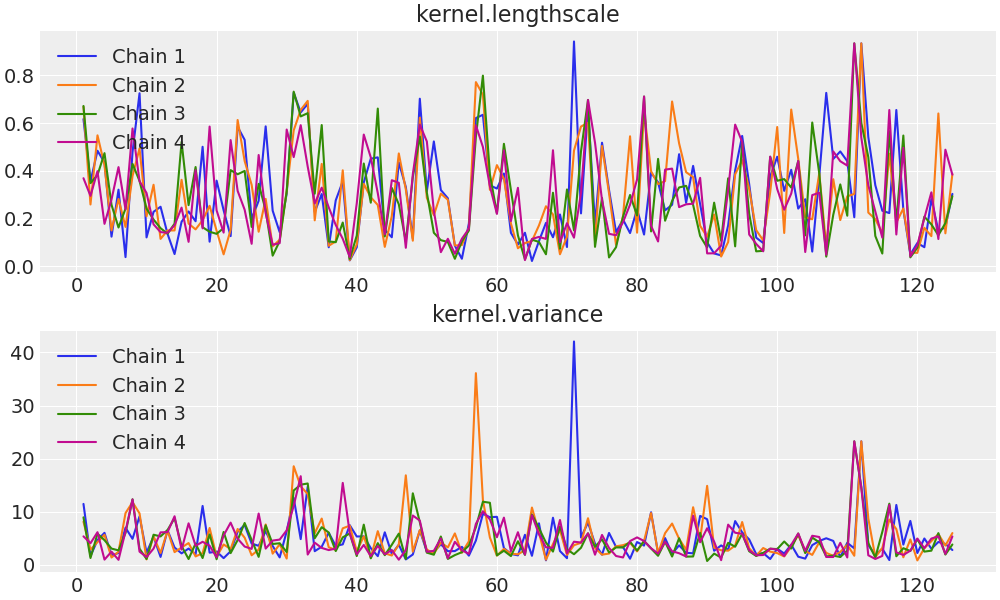
\includegraphics[width=0.5\textwidth]{src/traceplots.png}
    \caption{Trace plots of the Markov chains.}
    \label{fig:mcmc}
\end{figure}

\begin{table}[H]
\centering
\resizebox{\textwidth}{!}{\begin{tabular}{lrrrrrrrrr}
\toprule
{} &   mean &     sd &  hdi\_2.5\% &  hdi\_97.5\% &  mcse\_mean &  mcse\_sd &  ess\_bulk &  ess\_tail &  r\_hat \\
\midrule
kernel.lengthscale &  0.294 &  0.191 &     0.022 &      0.657 &      0.017 &    0.012 &     111.0 &     247.0 &   1.01 \\
kernel.variance    &  4.792 &  4.144 &     0.743 &     11.903 &      0.314 &    0.222 &     206.0 &     135.0 &   1.01 \\
\bottomrule
\end{tabular}}
\caption[]{Diagnostics of MCMC samples generated by NUTS.}
\label{tab:mcmc}
\end{table}

Based on the diagnostics in \autoref{appendix2}, we obtain our final 500 samples from $p(\bm{\theta}|\mathcal{D})$ using four chains, but this time with a warm-up period of 10 for each chain. Diagnostics for our final sample is given in \autoref{fig:mcmc} and \autoref{tab:mcmc} A scatter plot of the samples on log-log-scale is given \autoref{fig:loglog} and a plot of the posterior predictive is given in \autoref{fig:postpred}.

\begin{figure}[H]
        \centering
        \begin{subfigure}[b]{0.475\textwidth}
            \centering
            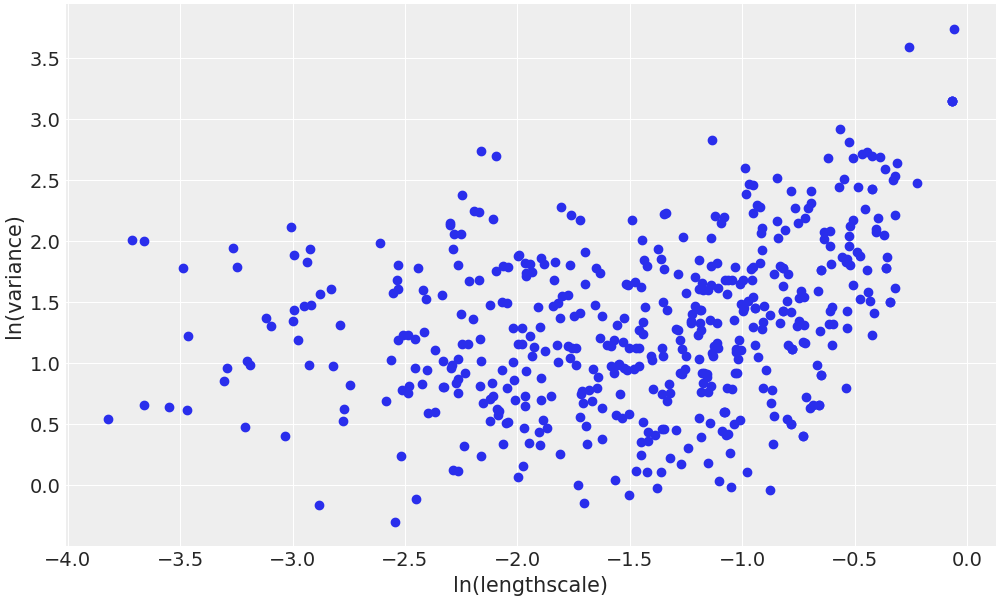
\includegraphics[width=\textwidth]{src/loglogplot.png}
            \caption{}
            \label{fig:loglog}
        \end{subfigure}
        \hfill
        \begin{subfigure}[b]{0.475\textwidth}  
            \centering 
            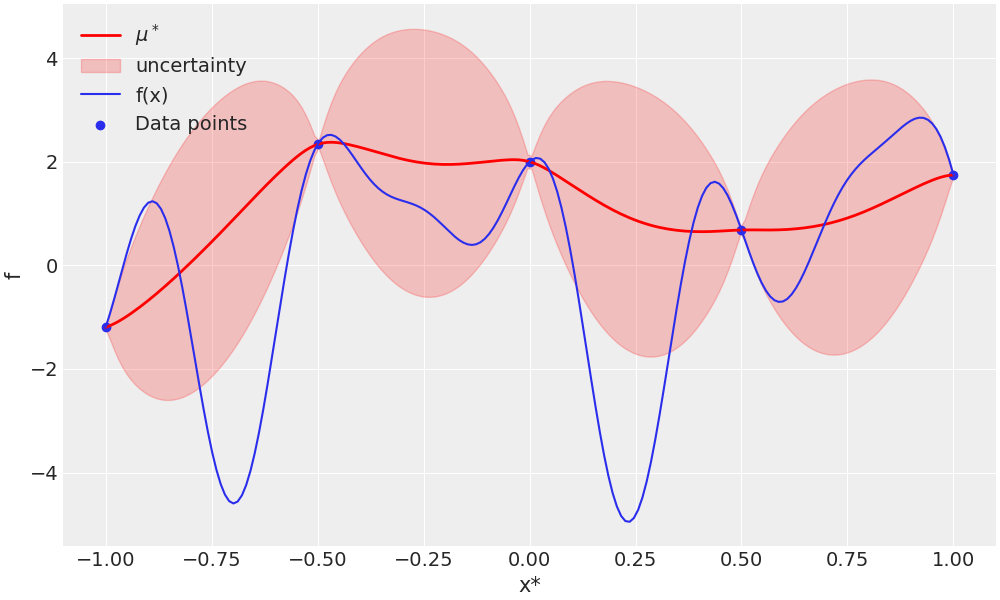
\includegraphics[width=\textwidth]{src/posteriorpred.png}
            \caption{}
            \label{fig:postpred}
        \end{subfigure}
        \caption[]
        {(a) Scatter plot on log-log scale of $N=500$ samples from $p(\bm{\theta}|\mathcal{D})$, (b) $p(f^*|x^*,\mathcal{D})$ for $x^*\in[-1, 1]$.} 
        \label{fig:targetsmulti}
    \end{figure}


\subsection*{B.2 – Bayesian Optimization}

\subsubsection*{Deliverable 1 \& 2}
We consider algorithm 1 in a setting with $T=50$ iterations and $n=20$ repetitions. To ensure convergence of the MCMC chain to its stationary distribution, we deem that a warm-up period of 10 samples is sufficient. We show the sampled $f^*$ at iterations $k=$0, 5, 10 in \autoref{fig:algorithm1} and \autoref{fig:performance1}, and \autoref{tab:avgiter} provide a summary of the above setting.

\begin{figure}[H]
    \centering
    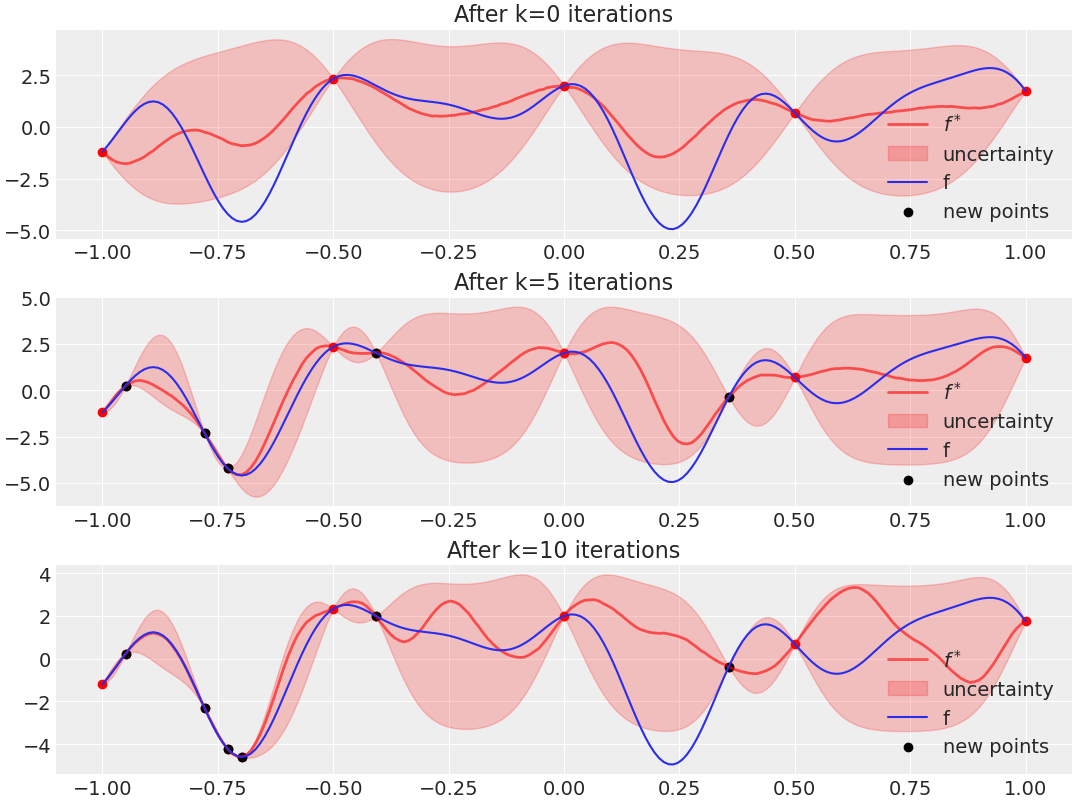
\includegraphics[width=0.5\textwidth]{src/algorithm1plot.png}
    \caption{Sampled $f^*$, $f$, and  $p(f^*|x^*,\mathcal{D}, \bm{\theta}^{(k)})$ at $k=$0,5,10 iterations.}
    \label{fig:algorithm1}
\end{figure}
By inspection of \autoref{fig:performance1} we note that algorithm 1 (denoted alg\_1\_RBF) did not manage to find global optimum in 7 out of 50 repetitions, which is indicated by values of zero. In particular, the decision rule implies that the algorithm in some repetitions becomes overconfident in regions with local optima. Thus, there is a very low probability that values of the sampled $f^*$ in the region of the global optimum will lie below the value of the sampled $f^*$ in the region of the local optimum, and hence a low probability that the algorithm will explore the region of the global optimum. This is evident from \autoref{fig:algorithm1}, where the probability that the sampled value of $f^*$ in the region of the global optimum attains a value that lies below the sampled value of $f^*$ in the region of the local optimum is less than 0.025\footnote{Values two standard deviations above the mean are not relevant, hence 0.025.}. This can be deduced by noting that $f^*$ in the region of the global optimum must attain a value that lies more than two standard deviations away from the mean. 

\subsubsection*{Deliverable 3}
One immediate extension to ensure that the algorithm eventually will find the global minimum is to not allow for repeated decisions in terms of the added point, $(x_p^*, f(x_p^*))$. In this way, the algorithm is forced to explore alternative optima by considering the optimal point among the set of points, in which the previous sampled points are not included. Since $f(x)$ is assumed to be noiseless, no information is gained by resampling the same point. We denote this algorithm 1.1.\\
Another alternative is to incorporate the information contained in $p(f^*|x^*,\mathcal{D},\bm{\theta}^{(i)})$ directly into the decision rule. One way to do so is the GP-LCB algorithm proposed by \cite{Srinivas_2012}, where the decision rule is given by:
\begin{equation}
    x_p^* = \argmin_i \left\{ \mu_{\bm{\theta}}^*(x_i^*) - \sqrt{\beta}_k \sigma_{\bm{\theta}}^*(x_i^*)\right\}, \qquad \beta_k = \phi\cdot\ln(k)
\end{equation}
Where $\phi$ is a confidence parameter. GP-LCB follows the 'optimism in face of uncertainty principle', in which we choose optimistic candidate points taking into account the variance of the GP. Note, however, that the success of the algorithm crucially relies on $\beta_k$ being increasing as a function of $\ln(k)$. Otherwise, GP-LCB will run into the same pitfalls as algorithm 1. Likewise, if $\phi$ is set too low, GP-LCB will become overconfident and get stuck in local optima for many iterations\footnote{On the other hand, it should also not be set too high so that the algorithm is too exploratory. In either case, it will converge to the optimum eventually as long as $\beta_k$ is increasing as a function of $\ln(k)$.}. Intuitively, when $\beta_k$ increases as a function of $\ln(k)$, $\sqrt{\beta_k}\sigma_{\bm{\theta}}^*(x^*)$ evaluated in regions with high uncertainty will eventually become larger than the $\sqrt{\beta_k}\sigma_{\bm{\theta}}^*(x^*)$ evaluated in regions with low uncertainty, since the magnitude of $\sigma_{\bm{\theta}}^*(x^*)$ will be larger in regions with higher uncertainty. In this way it is ensured that GP-LCB will never become overconfident in local optima regions, as it will eventually explore regions with higher uncertainties.\\
Another way to make the algorithms more exploratory can be induced by choosing a kernel with higher uncertainty estimates either through the kernel type itself or through the prior for the hyperparameters. The exploratory nature of our sampled $f^*$ from $p(f^*|x^*,\mathcal{D}, \bm{\theta}^{(k)})$ is primarily determined by the sampled $\bm{\theta}^{(k)}$ from $p(\bm{\theta}|\mathcal{D})$. That is, if we compare the behaviour of $f^*$ using a Matérn 3/2 kernel, it will explore much of the same space as with a RBF kernel for most of the sampled values from $p(\bm{\theta}|\mathcal{D})$ (which is also suggested by the results in \autoref{fig:performanceplots}). Thus, we induce more exploration by introducing a new prior, $\sigma_\mathit{s}^2\sim\text{LogNormal}(1.7, 0.3)$, and use a Matérn 3/2 kernel as a robustness check. \autoref{fig:performanceplots} and \autoref{tab:avgiter} provide a summary of the experiment with $\phi=2$. Evidently, a prior favoring larger values of $\sigma_\mathit{s}^2$ can by itself alleviate the issue of algorithm 1 getting stuck in local optima.

\begin{figure}[H]
        \centering
        \begin{subfigure}[b]{0.475\textwidth}
            \centering
            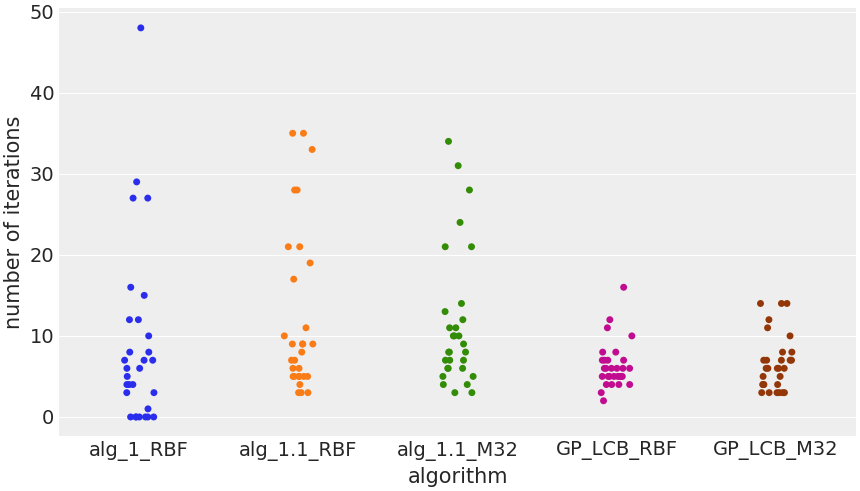
\includegraphics[width=\textwidth]{src/performanceplotorignalprior.png}
            \caption{}
            \label{fig:performance1}
        \end{subfigure}
        \hfill
        \begin{subfigure}[b]{0.475\textwidth}  
            \centering 
            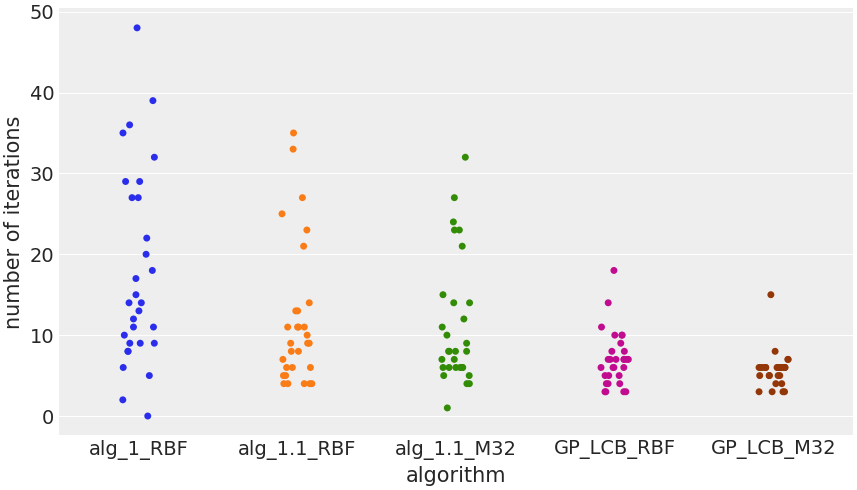
\includegraphics[width=\textwidth]{src/performanceplotsnewprior.png}
            \caption{}
            \label{fig:performance2}
        \end{subfigure}
        \caption[]
        {Number of iterations until global minimum is found. 0 iterations indicate that the that the global is never found. (a) With $\sigma_\mathit{s}^2\sim\text{LogNormal}(0, 2)$ (b) With $\sigma_\mathit{s}^2\sim\text{LogNormal}(1.7, 0.3)$.} 
        \label{fig:performanceplots}
    \end{figure}

\begin{table}[H]
\centering
\resizebox{\textwidth}{!}{\begin{tabular}{llllllr}
\toprule
  &  alg\_1\_RBF & alg\_1.1\_RBF & alg\_1.1\_M32 & GP\_LCB\_RBF &  GP\_LCB\_M32 \\
\midrule
 $\sigma_\mathit{s}\sim\text{LogNormal}(0, 2)$ & 20.63 &  12.36  &   11.53 &   6.33 &  6.67 \\
 $\sigma_\mathit{s}\sim\text{LogNormal}(1.7, 0.3)$ & 19.50 &  11.87  &   11.20 &   7.00 &  5.73 \\
\bottomrule
\end{tabular}}
\caption[]{Average number of iterations until global minimum is found. Note that alg\_1\_RBF counts 50 iterations in the average when the global minimum is not found.}
\label{tab:avgiter}
\end{table}

\iffalse

\newpage
\textbf{I praksis giver Matern kernel ikke meget mere uncertainty end RBF kernel (på trods af Oswins script indikerer det). Det afhænger i højere grad af sampled lengthscale og sampled variance. Derfor er følgende lidt forkert. }For instance, choosing $\kappa=1$ will produce good results with a Matérn 5/2 kernel, but poor results with a RBF kernel. On the other hand, choosing $\kappa=4$ will produce opposite results, as the Matérn 5/2 kernel induces too much exploration. Note however, that since we found that algorithm 1 wasn't exploratory enough, a Matérn 5/2 kernel by itself can improve algorithm 1. \textbf{I og med der ikke er nogen $\phi$-parameter i algorithm 1, så kan Matern kernel 5/2 i sig selv hjælpe betydeligt på algoritme 1, da den inducerer højere varians, og dermed mere exploratory!!}\\
Summary statistics for our preferred choice of GP-LCB initialization using the RBF kernel is given in table ?.\\
table/figure here\
\fi

\iffalse
Since we are investigating the predictive posterior we need to only sample a single from the posterior of the parameters $p(\bm{\theta} \vert \mathcal{D})$, however, this does not imply we can sample a single point in each iteration, get a new data point and $(x^*_p, y^*_p)$, and run a single iteration of the Markov chain to get a new sample of the posterior. This is due to two reasons. First, the samples from the posterior $p(\bm{\theta} \vert \mathcal{D})$ needs to be \textit{i.i.d}, to be representative samples when sampling the predictive posterior. However, Markov chains does in practice show a degree of auto-correlation between samples, so the chain needs to run for some time between two draws to ensure, that the samples from the posterior in fact are  \textit{i.i.d.} Second point is, that $f^*$ do need to be sampled from the posterior of $f^* \sim p(f^* \vert X, \mathcal{D})$. We need to take into account, that the dataset $\mathcal{D}$ is updated, that is $\mathcal{D} \leftarrow \mathcal{D} \cup \{(x^*_p, y^*_p)\}$, why we need to run the Markov chain to update the posterior once more.

\textbf{Deliverable 1:}

\textbf{Deliverable 2:}

\textbf{Deliverable 3:} As alluded to in the question, there are 3 obvious approaches to improve the algorithm. 1) kernel SKRIV. 2) prior SKRIV. 3) We can consider, if there are more efficient ways to search for points. Since the setup in this assignment requires us to consider 200 evenly spaced index points in the interval $[-1, 1]$, two obvious considerations can be made. First, and the most simple way to improve the algorithm is to remove already investigated points. Since we have fixed the variance of $y$ to be very small (non existent), then, when we have evaluated a point in $f(\cdot) $ a single time, we have ground truth of the specific point. In other words, if we again would redraw that point, we cannot gain any additional information. Second thing to consider is, how we trade off exploitation and exploration. We can very easily end up in a region of the optimization problem, where we have low expected outcome, and keep exploiting this region. We therefore need to employ an algorithm that let us efficiently search over not just a local maximum put the entire search space. For this we choose the online learning approach called Gaussian Process Lower Confidence Bound (CITÉR SRINIVASAN 2012). Formally this implies:

\begin{equation}
    x_i^* = argmin \left\{ \mu(x_i) - \sqrt{\beta}_t \sigma(x_i)\right\}, \qquad \beta_t = g(\ln(t), \kappa)
\end{equation}

where $\kappa$ is a set of hyper parameters.

\fi